\documentclass[journal]{vgtc}                % final (journal style)
%\documentclass[review,journal]{vgtc}         % review (journal style)
%\documentclass[widereview]{vgtc}             % wide-spaced review
%\documentclass[preprint,journal]{vgtc}       % preprint (journal style)

%% Uncomment one of the lines above depending on where your paper is
%% in the conference process. ``review'' and ``widereview'' are for review
%% submission, ``preprint'' is for pre-publication, and the final version
%% doesn't use a specific qualifier.

%% Please use one of the ``review'' options in combination with the
%% assigned online id (see below) ONLY if your paper uses a double blind
%% review process. Some conferences, like IEEE Vis and InfoVis, have NOT
%% in the past.

%% Please use the ``preprint''  option when producing a preprint version
%% for sharing your article on an open access repository

%% Please note that the use of figures other than the optional teaser is not permitted on the first page
%% of the journal version.  Figures should begin on the second page and be
%% in CMYK or Grey scale format, otherwise, colour shifting may occur
%% during the printing process.  Papers submitted with figures other than the optional teaser on the
%% first page will be refused. Also, the teaser figure should only have the
%% width of the abstract as the template enforces it.

%% These few lines make a distinction between latex and pdflatex calls and they
%% bring in essential packages for graphics and font handling.
%% Note that due to the \DeclareGraphicsExtensions{} call it is no longer necessary
%% to provide the the path and extension of a graphics file:
%% 
\includegraphics{diamondrule} is completely sufficient.
%%
\ifpdf%                                % if we use pdflatex
  \pdfoutput=1\relax                   % create PDFs from pdfLaTeX
  \pdfcompresslevel=9                  % PDF Compression
  \pdfoptionpdfminorversion=7          % create PDF 1.7
  \ExecuteOptions{pdftex}
  \usepackage{graphicx}                % allow us to embed graphics files
  \DeclareGraphicsExtensions{.pdf,.png,.jpg,.jpeg} % for pdflatex we expect .pdf, .png, or .jpg files
\else%                                 % else we use pure latex
  \ExecuteOptions{dvips}
  \usepackage{graphicx}                % allow us to embed graphics files
  \DeclareGraphicsExtensions{.eps}     % for pure latex we expect eps files
\fi%

%% it is recomended to use ``\autoref{sec:bla}'' instead of ``Fig.~\ref{sec:bla}''
\graphicspath{{figures/}{pictures/}{images/}{./}} % where to search for the images

\usepackage{microtype}                 % use micro-typography (slightly more compact, better to read)
\PassOptionsToPackage{warn}{textcomp}  % to address font issues with \textrightarrow
\usepackage{textcomp}                  % use better special symbols
\usepackage{mathptmx}                  % use matching math font
\usepackage{times}                     % we use Times as the main font
\renewcommand*\ttdefault{txtt}         % a nicer typewriter font
\usepackage{cite}                      % needed to automatically sort the references
\usepackage{tabu}                      % only used for the table example
\usepackage{booktabs}                  % only used for the table example
%% We encourage the use of mathptmx for consistent usage of times font
%% throughout the proceedings. However, if you encounter conflicts
%% with other math-related packages, you may want to disable it.

\usepackage[table]{xcolor}
\usepackage{floatrow}                % for organizing figures
\usepackage{breqn}                   % for multi-line equations

%% In preprint mode you may define your own headline. If not, the default IEEE copyright message will appear in preprint mode.
%\preprinttext{To appear in IEEE Transactions on Visualization and Computer Graphics.}

%% In preprint mode, this adds a link to the version of the paper on IEEEXplore
%% Uncomment this line when you produce a preprint version of the article 
%% after the article receives a DOI for the paper from IEEE
%\ieeedoi{xx.xxxx/TVCG.201x.xxxxxxx}

%% If you are submitting a paper to a conference for review with a double
%% blind reviewing process, please replace the value ``0'' below with your
%% OnlineID. Otherwise, you may safely leave it at ``0''.
\onlineid{0}

%% declare the category of your paper, only shown in review mode
\vgtccategory{Research}
%% please declare the paper type of your paper to help reviewers, only shown in review mode
%% choices:
%% * algorithm/technique
%% * application/design study
%% * evaluation
%% * system
%% * theory/model
\vgtcpapertype{application/design study}

%% Paper title.
\title{Understanding Urban Behavior Using Taxi Trips}

%% This is how authors are specified in the journal style

%% indicate IEEE Member or Student Member in form indicated below
\author{Nafiul Nipu, Ishan Choudhary,  Thiruvenkadam S  Radhakrishnan}
\authorfooter{
%% insert punctuation at end of each item
Email - mnipu2@uic.edu, ichoud6@uic.edu, tsivap2@uic.edu

}

%other entries to be set up for journal
\shortauthortitle{Biv \MakeLowercase{\textit{et al.}}: Global Illumination for Fun and Profit}
%\shortauthortitle{Firstauthor \MakeLowercase{\textit{et al.}}: Paper Title}

%% Abstract section.
%\abstract{Duis autem vel eum iriure dolor in hendrerit in vulputate
%velit esse molestie consequat, vel illum dolore eu feugiat nulla
%facilisis at vero eros et accumsan et iusto odio dignissim qui blandit
%praesent luptatum zzril delenit augue duis dolore te feugait nulla
%facilisi. Lorem ipsum dolor sit amet, consectetuer adipiscing elit,
%sed diam nonummy nibh euismod tincidunt ut laoreet dolore magna
%aliquam erat volutpat. Ut wisi enim ad minim veniam, quis nostrud exerci tation ullamcorper
%suscipit lobortis nisl ut aliquip ex ea commodo consequat. Duis autem
%vel eum iriure dolor in hendrerit in vulputate velit esse molestie
%consequat, vel illum dolore eu feugiat nulla facilisis at vero eros et
%accumsan et iusto odio dignissim qui blandit praesent luptatum zzril
%delenit augue duis dolore te feugait nulla facilisi.%
%} % end of abstract

%% Keywords that describe your work. Will show as 'Index Terms' in journal
%% please capitalize first letter and insert punctuation after last keyword
%% \keywords{Radiosity, global illumination, constant time}

%% ACM Computing Classification System (CCS). 
%% See <http://www.acm.org/class/1998/> for details.
%% The ``\CCScat'' command takes four arguments.

%% \CCScatlist{ % not used in journal version
%% \CCScat{K.6.1}{Management of Computing and Information Systems}%
%% {Project and People Management}{Life Cycle};
%% \CCScat{K.7.m}{The Computing Profession}{Miscellaneous}{Ethics}
%% }

%% A teaser figure can be included as follows
%\teaser{
%  \centering
%  \includegraphics[width=\linewidth]{CypressView}
%  \caption{In the Clouds: Vancouver from Cypress Mountain. Note that the teaser may not be wider than the abstract block.}
%  \label{fig:teaser}
%}

%% Uncomment below to disable the manuscript note
\renewcommand{\manuscriptnotetxt}{}

%% Copyright space is enabled by default as required by guidelines.
%% It is disabled by the 'review' option or via the following command:
% \nocopyrightspace


\vgtcinsertpkg
\raggedbottom
%%%%%%%%%%%%%%%%%%%%%%%%%%%%%%%%%%%%%%%%%%%%%%%%%%%%%%%%%%%%%%%%
%%%%%%%%%%%%%%%%%%%%%% START OF THE PAPER %%%%%%%%%%%%%%%%%%%%%%
%%%%%%%%%%%%%%%%%%%%%%%%%%%%%%%%%%%%%%%%%%%%%%%%%%%%%%%%%%%%%%%%%

\begin{document}

%% The ``\maketitle'' command must be the first command after the
%% ``\begin{document}'' command. It prepares and prints the title block.

%% the only exception to this rule is the \firstsection command
% \firstsection{Introduction}

\maketitle


\section{Introduction}
Now-a-days cities offer massive flux of economic and human development opportunities owing to the rapid advancement in urbanization. These opportunities lead to more people migrating to in cities. As more people are bound towards cities, there has been a massive increase in traffic, social events and environmental side-effects, thereby placing more importance on city planning to better manage these factors. Due to the advancement in technology, city officials can automatically collect a large amount of data related to urban behaviors. In recent years, city officials have made these data sets available publicly to research and analyze in order to understand different aspects of urban planning, development and behaviors.

From the different urban datasets available, taxi trips data is one of the most popular and researched as they not only provide valuable information of people's movements through the city in terms of pickups and drop-offs. Hence, it is possible to answer questions about popular places, tourist hotspots and so on by carefully examining taxi data. In particular, in this work, we are interested in identifying such hotspots over time with the help of taxi trip data. After identifying the hotspots we aim to explain the reason for those hotspots. In order to explain such events, we look into social media conversations; specifically Twitter data. Twitter data provides us with a unique perspective as people use the social media platform to discuss their daily activities and share their opinions.

We detail a well rounded framework to detect such hotspots from Taxi data and use this information as spatio-temporal constraints in analyzing the Twitter conversations. In addition, we propose a visual analytics system that can be used to explore these datasets and understand the change in urban behavior.
 


\section{Related Work}
% taxi data research
Due to the availability of important information in open taxi data, a lot of research has focused on analyzing them to gain valuable insights. Ge et al. \cite{ge2010energy} proposed a mobile recommender system that recommends taxi drivers potential pick-up and parking positions to maximize business success and minimize energy consumption. Ferreira et al. \cite{ferreira2013visual} proposed a visual system that allows users to make Spatio-temporal queries of taxi trips to visually explore and compare the results. Their proposed system takes into account a large number of taxi data and offers a scalable and efficient solution. Numerous research has been conducted analyzing taxi data from various cities including Lisbon \cite{veloso2011exploratory}, Beijing \cite{liang2012scaling}, Shanghai \cite{peng2012collective}, and so on. These analyses are focused on explaining the taxi pickup and dropoff locations with different city contexts. However, none of these works considered explaining why there might be a sudden change in taxi trips in terms of environmental aspects. In contrast, we concentrate on finding the reason behind this phenomenon with the help of different scenarios such as changes in urban planning, events, and news.  


% %pluto data research
% 	Numerous researchers have tried to analyze different aspects of urban planning of New York City using the rich PLUTO data or with the complementary spatio-temporal Map Pluto data in different use cases. Yuquin et al  \cite{yuqin2021spatio} used PLUTO data along with geotagged social media data to analyze how COVID-19 affected human mobility patterns by land-use types such as residential, commercial, and workplaces, etc. Yang et al.  \cite{yang2021urban} used the correlation between building density in a tax lot area and demographic information and public transit data to understand how urban density, commuting, and economic inequalities affected the infection rates during the pandemic. With our visual system, we aim to look beyond the impact of the pandemic and generalize the effect of social and other events on mobility by also leveraging additional datasets such as taxi data and social media data.
	

% sentiment analysis research
Pang et al. \cite{bo2008opinion} surveyed the significance of sentiment analysis in its early years in and since its research has grown tremendously over the past couple of years. The number of papers published in the field has grown exponentially in recent years, from 37 papers in the year 2000 to 5,699 papers in a matter of 15 years. While earlier algorithms have focused on lexicon-based analysis \cite{maite2011lexicon}, more recent algorithms have focused on machine learning and deep learning. These learning methods have produced excellent results given the pervasiveness of copious amounts of data in modern times. Mäntylä et al \cite{M_ntyl__2018} discussed various modern tools and techniques in sentiment analysis. In addition, there are several APIs providing sentiment analysis capabilities such as Microsoft Text Analytics API, AYLIEN Text Analysis API, Senti API, et cetera. 


%analyzing daily activities
Over the years, there have been many works related to analyzing and understanding daily human activities. Much of this research focuses on data gathered from social networking sites such as Twitter. Social networking sites prove to be a  useful resource for gathering information about human activities as people express and share their thoughts and opinions through them \cite{giachanou2016like}. However, most of the works focus on analyzing public sentiments using Twitter data. In contrast, we direct our analysis on using the sentiment to define and explain certain activities related to the taxi trips.


Overall, none of the existing works of literature have correlated their respective fields with taxi data to gain insights. Our work aims to find significant correlations between each of these above-mentioned domains to determine societal behavior.

\section{Data description}

In this section, we present a brief description of the data that we plan to analyze using our proposed visual system. 

\textbf{Taxi Trip Data :} NYC taxi trip data is spatio-temporal multivariate data. The data consists of monthly taxi trip details of three types of taxi - Yellow, Green, For-hire over the years. Each monthly trip data consists of the location of the pickup and dropoff points for each trip. Datasets are huge. For this work, we took into consideration three months of Taxi trips data from October to December, 2018. Each month consists information of approximately 30M of taxi trips. 

\textbf{Twitter Data :} Twitter data has been used in Sentiment classification;  a well-researched topic. In this project, our aim is to build a general sentiment classifier and utilize that to analyze Twitter data over popular news articles to predict the general public sentiment resulting from them. In addition to sentiment classifier we also propose a topic modeling algorithm to extract relevant topics related to various events such as Halloween, Thanksgiving and so on. For the analysis, we used NYC twitter data from October to December, 2018. Each month consists of around 1.2M tweets. The topic and public sentiment derived from these classified tweets are then used to correlate urban taxi trip behavior. In general, the Twitter data are spatio-temporal consisting of the actual tweet, time, and location. 


% To train our initial sentiment classifier, we will use the Kaggle Sentiment140 Dataset of 1.6 Million tweets and use that to classify relevant tweets extracted from the Twitter API. We plan to apply for the Academic Research Product track which allows users to download 10 million tweets a month. The public sentiment derived from classified tweets will then be used to correlate urban taxi trip behavior. 
\section{Research}

We aim to build a visual analytics system that can be used in understanding social behaviors and urban activities. This is done through two key steps, namely

\begin{itemize}
\item Extract events from taxi data
\item Analyze social media conversations corresponding to the events
\end{itemize}

Combining these two steps, we proposed a framework that can be used in interactively exploring different events around a city across time, using these observations to draw hypotheses and apply the findings in various fields.

\subsection{Analytical Frameworks}
In this section, we further detail the analytical frameworks that we used for the two key steps mentioned above.

\subsubsection{Taxi Data Analysis}
To extract events from the taxi data, we use Topological Data Analysis (TDA) to identify the maxima and minima events across the spatio-temporal data. Conneau et al. \cite{xlmroberta} used TDA to extract events from taxi data. Miranda et al. \cite{miranda2017Urban} also extracted urban pulses from scalar data of Flickr photo counts. First, we will aggregate the taxi data into a scalar function by applying a Gaussian kernel on it. Here, we use the total drop off in a particular latitude-longitude to create the aggregation so that we can explore other aggregations that might produce more meaningful results. For example, comparing the trends of total drop offs by date to the average deviation from weekday mean showed in (Fig.~\ref{fig:dailytrends}). It is clear that the latter might be able to identify more interesting events which might be produce better results for our use-case. However, this process will be explored further as our future work.

We then apply a lowerstar filter on top of the scalar image and compute the persistence of various events in the data. We filter out the events with the highest lifetime to identify the maxima events and map it back to a latitude-longitude. The same can be performed for a range of dates to identify all such events of interest from the spatio-temporal data. With this our first step is completed. This process is depicted visually in Fig.~\ref{fig:tda}. These experiments were carried out using the Ripser python TDA package \cite{ripser}.

\begin{figure}[ht]
 \centering % avoid the use of \begin{center}...\end{center} and use \centering instead (more compact)
 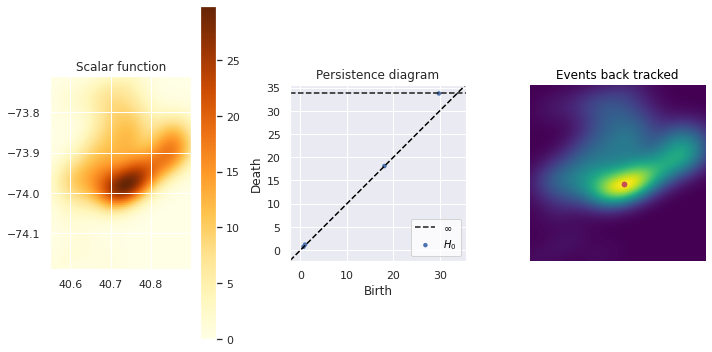
\includegraphics[scale=.25]{final/fig/TDA.png}
 \caption{Topological analysis of daily taxi trips}
 \label{fig:dailytrends}
\end{figure}


\subsubsection{Twitter Analysis}

Analyzing the twitter data entails two sub-tasks - 1. Topic modeling to understand what topics the conversations in specific areas are revolving around, 2. Sentiment analysis of these topics.

\textbf{Topic Modeling : }
We first explored the prevalent Latent Dirichlet Allocation algorithm, a probabilistic model that typically used for topic modeling. We used the Gensim \cite{gensim} python package for all experiments related to topic modeling. The general process of Topic modeling is the same as any natural language tasks and involves data cleaning (removing punctuation, stop words etc.), then lemmatization and finally feeding the documents (each instance of tweet here is referred to as a document) into a topic model. The LDA algorithm then iteratively trains on all these documents to model the representation of topics and their relation to the terms (i.e. words) present in the documents. Once trained, the model can be used to predict the topic present in a particular document as a probability distribution.

The joint probability in LDA is formulated as:

$${\delta = \prod_{d=1}^{D} p(\Theta_d|\alpha) 
\prod_{n=1}^{N} p(z_{d,n}|\Theta_d)p(w_{d,n}|\beta_{1:K},z_{d,n})}$$

$${p(\beta, \Theta, z | w) = \prod_{i=1}^{K} p(\beta_i | \eta) \delta
}$$

Where $\beta_k$ for a topic k is its word distribution, $\Theta$ is the topic proportions of a document, z is the topic assignment of a word, $\eta$ is the topic parameter and $\alpha$ is the proportions parameter.

We found that applying LDA had two key drawbacks. First, the topics and the key terms representing these topics were not known beforehand and remain static. The lack of dynamic change and addition of new key terms limits LDA's ability to model current events. Consequently, the coherence score of various iterations of the models were also poor (ranging between 30-50\%). Second, LDA is usually applied for documents of larger sizes, that produces more coherent topics. We also tried some workarounds by concatenating tweets from a day to produce a larger document, that did not improve the performance much. For these reasons, we moved on to explore an alternate methodology.

\begin{figure}[ht]
 \centering % avoid the use of \begin{center}...\end{center} and use \centering instead (more compact)
 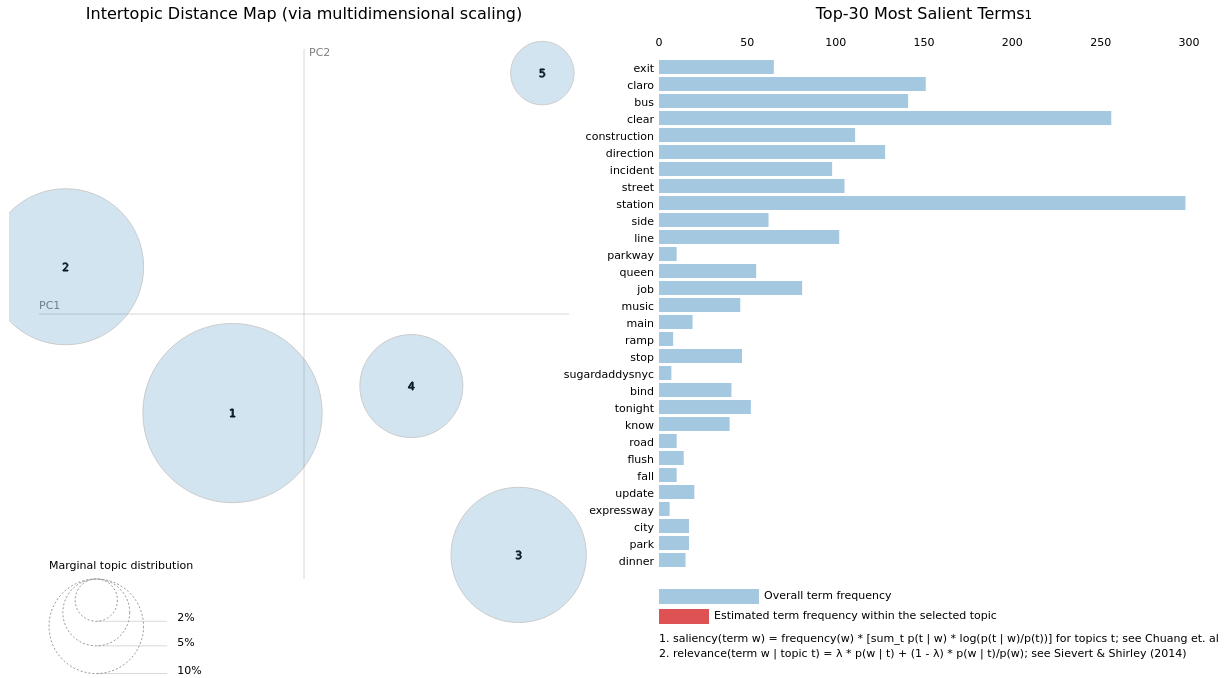
\includegraphics[scale=0.15]{final/fig/LDA.png}
 \caption{Topic Modeling results showing the created topics and their key terms to the right}
 \label{fig:tda}
\end{figure}

\textbf{Sentiment Analysis: }
In order to gain an understanding about the thoughts and associated feelings of users in our study, we required a tool to analyze the emotions behind posts made by each user. For this reason, we used data from the Twitter dataset and applied a discrete classification of sentiment into positive, negative and neutral in order to establish a suitable parameter to judge human feelings and behavior. 

In our first step, we cleaned and preprocessed the tweet using stemming, stop-word removal, and keyword extraction. Then, we applied the NLTK library`s sentiment classification on it to determine its respective scores for each sentiment. These scores would then be passed through a set threshold which helps us classify which sentiment a tweet belongs to.  Furthermore, besides classifying tweets, we also extracted general sentiment for each keyword for every hour, day and month respectively, thus allowing us to better analyse trends in sentiment change regrading any term over different duration. In our research, we emphasised on days with special events such as Halloween, Christmas, Thanksgiving and the New Year Eve.

While using NLTK provided us with a general sense of how users felt, we still felt the need for a more granular description of what the user felt to improve our analysis. In order to delve deeper and have more defined sentiments, we tried other approaches such as the Zero Shot Model which provided more depth and variations in the kinds of sentiment we could model. We will cover this in the next subsection.

\textbf{Zero Shot Model : }
In order to alleviate the drawbacks mentioned above we shifted from our initial task of Topic Modeling, to Topic Classification. As our analysis is mainly related to urban activity, we came up with some labels for topics such as ``Traffic/Construction'', ``Holiday/Celebration'', ``Politics'', ``Sports'', and other major seasonal events such as ``Halloween'', ``Thanksgiving'' and ``Christmas''.

We used a pre-trained language model that was trained on a multi-lingual dataset for a Natural Language Inference (NLI) task. NLI tasks have the setup of a premise and hypothesis and predicts whether the premise ``entails'', ``contradicts'', or is ``neutral'' to the hypothesis. We use the probability of ``entail''-ment as the probability of classification for the given labels. The underlying model is the XLM-RoBERTa language model\cite{xlmroberta} and we use the HuggingFace transformers pipeline to perform this inference.

One current drawback of this approach is that the inference takes a long time (~10 minutes for 10,000 tweets). We explored some parallel processing approaches to alleviate this with no success so far. We used this model for both Topic and Seniment classification (with labels such as - ``happy'', ``sad'', ``excited'' etc.)

\subsection{Implementation}

\subsubsection{System Architecture}
\begin{figure}[ht]
 \centering % avoid the use of \begin{center}...\end{center} and use \centering instead (more compact)
 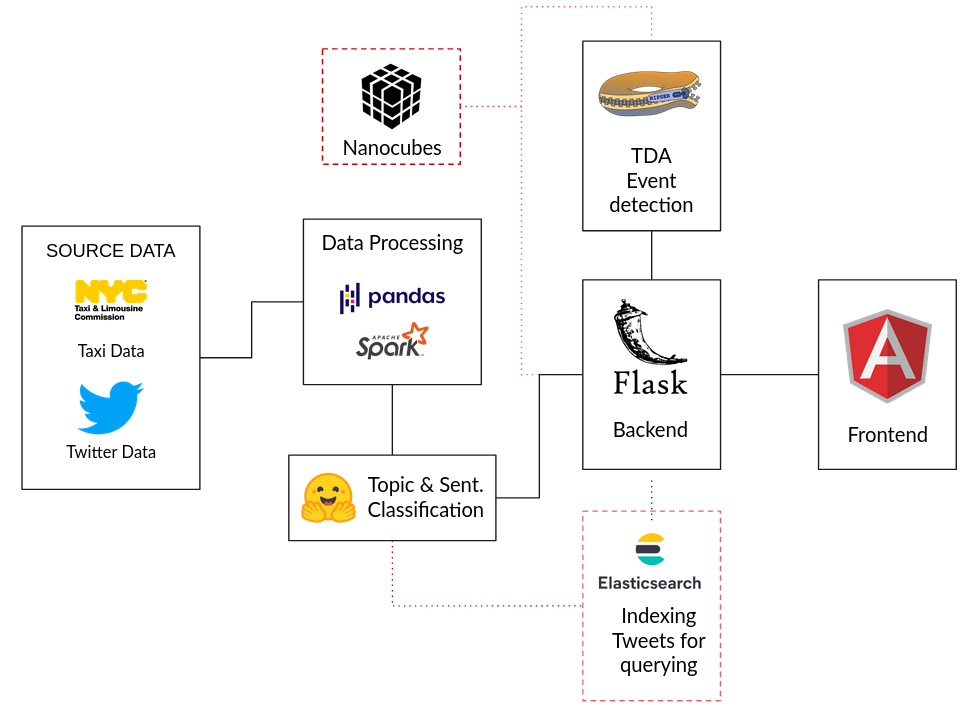
\includegraphics[width=\linewidth]{final/fig/system_arch.png}
 \caption{System architecture of the proposed visual analytics system}
 \label{fig:architecture}
\end{figure}


% \begin{figure*}[t]
% \centering
% \rule{\linewidth}{3cm}
% \caption{Wide single column figure in a twocolumn document.}
% \end{figure*}

We propose the following architecture for our visual analytics system  as depicted in (Fig.~\ref{fig:architecture})

There are three layers:
\begin{itemize}
    \item Source data:
        \begin{itemize}
            \item Consists of the three primary data sources - NYC Taxi trip data and Twitter data
            \item Data was be ingested from these sources through direct data pull, will be eventually automated to extract data for all available years
        \end{itemize}
        
    \item Data Management:
        \begin{itemize}
            \item In this layer, we performed the necessary cleaning and aggregation of taxi data at a daily level
            \item Pandas and Spark libraries were used to perform aggregation and to speed up the pre-processing steps such as mapping a tweet and taxi ride records to a specific taxi zones
            \item We also use the HuggingFace Zero-shot pipeline to infer topic and sentiment for all the tweets in this layer
            \item Additionally, we will perform TDA on the aggregated Taxi data to extract events of interest using the Ripser package
        \end{itemize}
    \item Visual System:
        \begin{itemize}
            \item The visual system is used to depict a visual representation of the extracted Taxi events and will allow for interactive exploration of selected events along with the topic and sentiment of the tweets corresponding to the selected event
            \item The system currently has an Angular front end and the Flask backend is a work in progress. Once functional, the Flask backed will serve the entire application and co-ordinate fetching information from the data management layer
        \end{itemize}
    \item Other Components:
        \begin{itemize}
            \item We also have two other components planned for the system that are yet to be explored
            \item We would use Nanocubes to serve aggregated Taxi data, to perform live event extraction on selected spatio-temporal constraints
            \item We would also use Elasticsearch to index and serve Tweets with their topics and sentiment to fetch results for a given constrains in a scalable manner
        \end{itemize}
\end{itemize}



\subsection{Task Analysis}
A description of the tasks are given below - 
\begin{itemize}
  \item Visualize big spatio-temporal data efficiently without any significant delay.
  \item What are the hotspots around the city throughout the different times of the year? What are the general trends and patterns in the taxi trips throughout the city?
  \item Identify any surge or drops in taxi pick-ups or drop-offs at certain locations in temporal space and explain the reason for such cases in terms of environmental change and social events
\end{itemize}
 
\subsection{Visual Interface}
\begin{figure}[ht]
 \centering % avoid the use of \begin{center}...\end{center} and use \centering instead (more compact)
 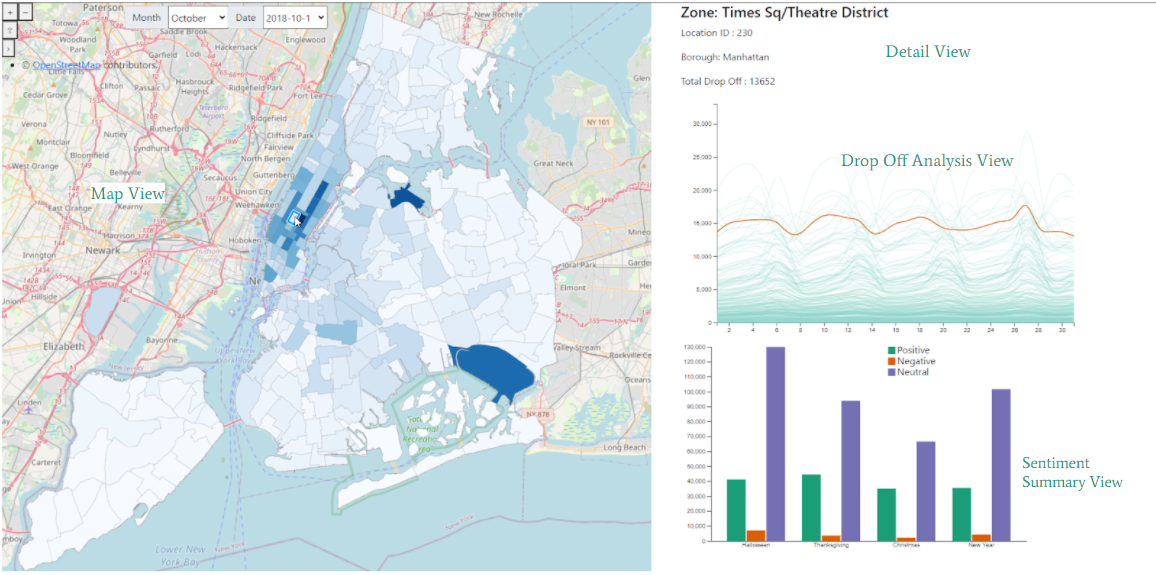
\includegraphics[width=\linewidth]{final/fig/interface.PNG}
 \caption{Visual interface of the proposed system}
 \label{fig:interface}
\end{figure}
We present a visual interface to to explore taxi and twitter data. The interface consists of four main views - Map view, Detail view, Drop Off Analysis View, Sentiment Summary view. 

\textbf{Map view} shows a heat map of New York City based on the taxi drop offs of NYC taxi zones for a selected date. User can select date and month from the dropdown menus. When user selects a zone from the map, the \textbf{detail view} shows relevant information such a zone name, location id, borough name and the drop off count. The \textbf{Drop Off Analysis View} shows the dropoff counts for a selected a month for all taxi zones. This view allows users to understand the change in drop offs over time. When user selects a zone from the map view, the selected zone is also highlighted in the dropoff analysis view. Finally, \textbf{Sentiment Summary View} shows the sentiments of the tweets based on topics such as Halloween, Thanksgiving, Christmas and so on.


\section{Results}
To analyze the effectiveness of our proposed methodology and visual system, we conducted three case studies. In this section we present the results of these three case studies. These case studies analyze three events that represent three types of abnormalities from the taxi data - increase in drop offs in a zone, decrease in drop offs in a zone, and a combination of both in two different zones.

\textbf{Case Study 1 - Halloween Week: } We first looked at the taxi-trends for the week of Halloween, and noticed an abnormal spike in the Civic center taxi zone (TriBeCa area) as seen in (Fig.~\ref{fig:tribecatrend}). To understand the potential motivation behind this, we looked at the topics and sentiment of the tweets from this taxi zone. There were significant proportion of tweets talking about Halloween (Celebration + Halloween topics) with almost all having a positive sentiment. We also noticed that people from the TriBeCa area tweeted ~6\% (14\% to 20\%) more during Halloween than during normal days. This indicated that there were many Halloween events happening in this zone that attracted people from different regions to the TriBeCa area. Further analysis can be done to understand the origin of people traveling to this zone for more observations.

\begin{figure}[h]
 \centering % avoid the use of \begin{center}...\end{center} and use \centering instead (more compact)
 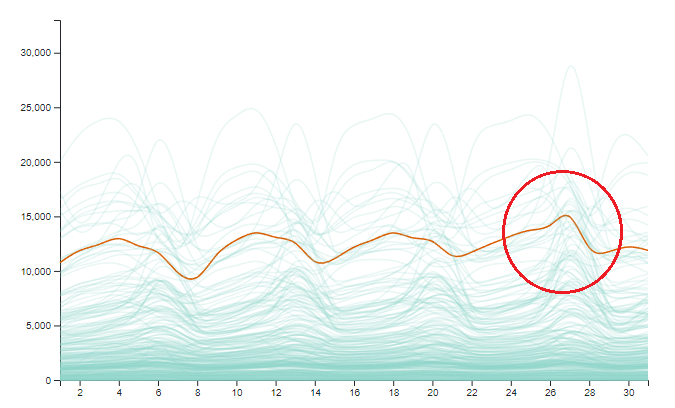
\includegraphics[width=\linewidth]{final/fig/Tribeca_taxi_trend.png}
 \caption{Trend of taxi drop offs by day in the TriBeCa zone}
 \label{fig:tribecatrend}
\end{figure}

Upon secondary research, it was understood that the TriBeCa area is widely popular for its Halloween events \cite{tribecanews} ranging from the long running tradition of Halloween Parade at the Washington Market Park to the events organized at the BMMC Tribeca Performing Arts Center which reinforced our hypothesis.


\textbf{Case Study 2 - Macy's Thanksgiving Parade: } This time, we noticed some decline in the number of drop-offs in the Logan Square East and Garment District zones during the Thanksgiving week. One of the major events that happens during this week is the Macy's parade. And it is typical for streets along the route of the parade to be closed down during this time and these two zones happen to be a part of the parade route. We also noticed that the ratio of tweets talking about the parade to the overall tweets from that region during the week was the highest for these two zones (~20\% tweets talking about the parade).

\begin{figure}[h]
 \centering % avoid the use of \begin{center}...\end{center} and use \centering instead (more compact)
 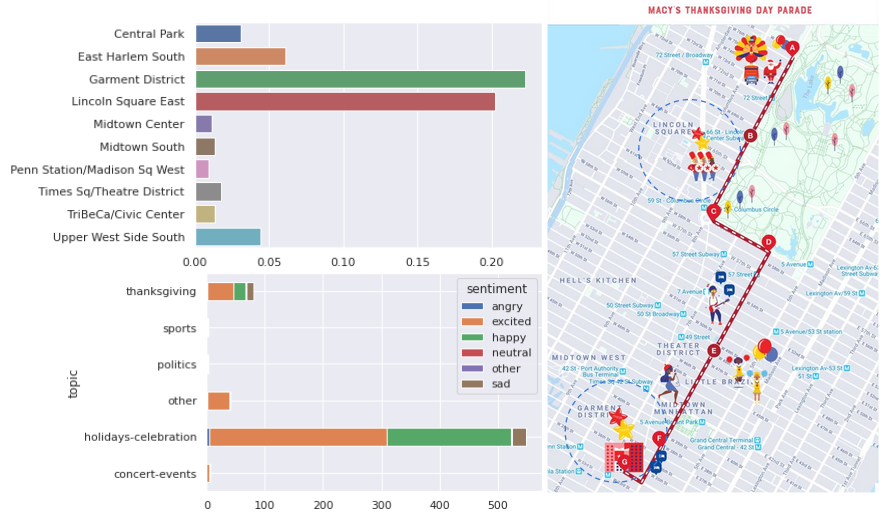
\includegraphics[width=\linewidth]{final/fig/Macys parade.png}
 \caption{Macy's parade route (right) and ratio of tweets talking about the parade by zone (top left)}
 \label{fig:macys}
\end{figure}

\textbf{Case Study 3 - Dec 31\textsuperscript{st} Celebration at Times Square: } For the final case study, we looked into the week of December 31\textsuperscript{st}. Here, from the Taxi data we noticed some abnormal increases in drop offs in the Clinton East zone and a sharp decline in drop offs in the Time Square zone. It is evident that the decline in the Time Square zone is due to the New Years celebration; the iconic Times Square ball drop event is widely famous around the world. Due to the event, the streets are typically closed off at the times square area. So naturally people look for a closer access point near Times Square, and Clinton East zone turns out to be one of those access points with streets offering entry into the Times Square area. Also, when we looked into the twitter data, we found a lot of conversations surrounding the traffic congestion as well.

These case studies confirm the effectiveness of the proposed framework of utilizing Taxi and Twitter data to understand urban movements and social behavior to some extent and raise other questions that can be explored further.

\section{Conclusion}
In this paper, we proposed a system that can extract relevant information from urban datasetes using topological framework, topic modeling and sentiment analysis. Additionally, we presented a visual analytics system to explore the taxi trips and twitter data. The visual interface will help the users to interactively explore the data and extract insights. Furthermore, we hypothesized exists a strong relation between taxi events and twitter conversations in that they contain information about urban behaviors. To support our hypothesis, we presented three case studies. More experiments can be done to further establish this relation. 

The zero-shot classifier provides better results compared to the traditional Topic modeling appraoches, however suffers from performance issues in terms of the time taken for inference. There is a workaround to distill the language network for inference on a set of labels using the teacher model that would make the process faster. We will explore this further.

In future, we want to experiment and analyze different scenarios and case studies to extract more concrete results. Additionally, we plan to make progress with the visual interface so that it can guide users with automatically detected events. Furthermore, better interactions will be provided to the users for ingesting the topic  and sentiment information of the tweets from selected constraints. 

Currently, our visual interface only handles three months of taxi and twitter data. We plan to make the visual system scalable so that it can handle larger amounts of data. Also, our drop off analysis view is visually cluttered and it can create a burden to the cognitive load of the users. Therefore, we will analyze and explore alternative approaches to reduce visual cluttering. Finally, this framework can be extended to pair any urban dataset along with Twitter data, such as the urban noise complaints data to extract events and understand urban behavior.

%\bibliographystyle{abbrv}
\bibliographystyle{abbrv-doi}
%\bibliographystyle{abbrv-doi-narrow}
%\bibliographystyle{abbrv-doi-hyperref}
%\bibliographystyle{abbrv-doi-hyperref-narrow}

\bibliography{final}
\end{document}

